%  LaTeX support: latex@mdpi.com 
%  For support, please attach all files needed for compiling as well as the log file, and specify your operating system, LaTeX version, and LaTeX editor.

%=================================================================
\documentclass[futureinternet,article,submit,pdftex,moreauthors]{Definitions/mdpi} 

%--------------------
% Class Options:
%--------------------
%----------
% journal
%----------
% Choose between the following MDPI journals:
% For posting an early version of this manuscript as a preprint, you may use "preprints" as the journal. Changing "submit" to "accept" before posting will remove line numbers.

%---------
% article
%---------

%----------
% submit
%----------
% The class option "submit" will be changed to "accept" by the Editorial Office when the paper is accepted. This will only make changes to the frontpage (e.g., the logo of the journal will get visible), the headings, and the copyright information. Also, line numbering will be removed. Journal info and pagination for accepted papers will also be assigned by the Editorial Office.

%------------------
% moreauthors
%------------------
% If there is only one author the class option oneauthor should be used. Otherwise use the class option moreauthors.

%---------
% pdftex
%---------
% The option pdftex is for use with pdfLaTeX. Remove "pdftex" for (1) compiling with LaTeX & dvi2pdf (if eps figures are used) or for (2) compiling with XeLaTeX.

%=================================================================
% MDPI internal commands - do not modify
\firstpage{1} 
\makeatletter 
\setcounter{page}{\@firstpage} 
\makeatother
\pubvolume{1}
\issuenum{1}
\articlenumber{0}
\pubyear{2024}
\copyrightyear{2024}
%\externaleditor{Academic Editor: Firstname Lastname}
\datereceived{ } 
\daterevised{ } % Comment out if no revised date
\dateaccepted{ } 
\datepublished{ } 
%\datecorrected{} % For corrected papers: "Corrected: XXX" date in the original paper.
%\dateretracted{} % For corrected papers: "Retracted: XXX" date in the original paper.
\hreflink{https://doi.org/} % If needed use \linebreak
%\doinum{}
%\pdfoutput=1 % Uncommented for upload to arXiv.org
%\CorrStatement{yes}  % For updates


%=================================================================
% Add packages and commands here. The following packages are loaded in our class file: fontenc, inputenc, calc, indentfirst, fancyhdr, graphicx, epstopdf, lastpage, ifthen, float, amsmath, amssymb, lineno, setspace, enumitem, mathpazo, booktabs, titlesec, etoolbox, tabto, xcolor, colortbl, soul, multirow, microtype, tikz, totcount, changepage, attrib, upgreek, array, tabularx, pbox, ragged2e, tocloft, marginnote, marginfix, enotez, amsthm, natbib, hyperref, cleveref, scrextend, url, geometry, newfloat, caption, draftwatermark, seqsplit
% cleveref: load \crefname definitions after \begin{document}

%PLACE TO ADD COMMANDS
\usepackage{lipsum}
\usepackage{algorithm}
\usepackage{algpseudocode}
\usepackage{subcaption}

%=================================================================
% Please use the following mathematics environments: Theorem, Lemma, Corollary, Proposition, Characterization, Property, Problem, Example, ExamplesandDefinitions, Hypothesis, Remark, Definition, Notation, Assumption
%% For proofs, please use the proof environment (the amsthm package is loaded by the MDPI class).

%=================================================================
% Full title of the paper (Capitalized)
\Title{AI-Based Detection of Jamming Attacks In 6G Drone Networks}

% MDPI internal command: Title for citation in the left column
\TitleCitation{AI-Based Detection of Jamming Attacks in 6G Drone Networks}

% Author Orchid ID: enter ID or remove command
\newcommand{\orcidauthorA}{0000-0000-0000-000X} % Add \orcidA{} behind the author's name
%\newcommand{\orcidauthorB}{0000-0000-0000-000X} % Add \orcidB{} behind the author's name

% Authors, for the paper (add full first names)
\Author{Sergio Cibecchini $^{1,\dagger,\ddagger}$\orcidA{}, Francesco Chiti $^{2,\ddagger}$ and Laura Pierucci$^{2,}$*}

%\longauthorlist{yes}

% MDPI internal command: Authors, for metadata in PDF
\AuthorNames{Sergio Cibecchini, Francesco Chiti and Laura Pierucci}

% MDPI internal command: Authors, for citation in the left column
\AuthorCitation{Cibecchini, S.; Chiti, F.; Lastname, F.}
% If this is a Chicago style journal: Lastname, Firstname, Firstname Lastname, and Firstname Lastname.

% Affiliations / Addresses (Add [1] after \address if there is only one affiliation.)
\address{%
$^{1}$ \quad Affiliation 1; e-mail@e-mail.com\\
$^{2}$ \quad Affiliation 2; e-mail@e-mail.com}

% Contact information of the corresponding author
\corres{Correspondence: sergio.cibecchini@gmail.com; Tel.: (optional; include country code; if there are multiple corresponding authors, add author initials) +xx-xxxx-xxx-xxxx (F.L.)}

% Current address and/or shared authorship
\firstnote{Current address: Affiliation.}  % Current address should not be the same as any items in the Affiliation section.
\secondnote{These authors contributed equally to this work.}
% The commands \thirdnote{} till \eighthnote{} are available for further notes

%\simplesumm{} % Simple summary

%\conference{} % An extended version of a conference paper

% Abstract (Do not insert blank lines, i.e. \\) 
\abstract{A single paragraph of about 200 words maximum. For research articles, abstracts should give a pertinent overview of the work. We strongly encourage authors to use the following style of structured abstracts, but without headings: (1) Background: place the question addressed in a broad context and highlight the purpose of the study; (2) Methods: describe briefly the main methods or treatments applied; (3) Results: summarize the article's main findings; (4) Conclusions: indicate the main conclusions or interpretations. The abstract should be an objective representation of the article, it must not contain results which are not presented and substantiated in the main text and should not exaggerate the main conclusions.}

% Keywords
\keyword{keyword 1; keyword 2; keyword 3 (List three to ten pertinent keywords specific to the article; yet reasonably common within the subject discipline.)} 

% The fields PACS, MSC, and JEL may be left empty or commented out if not applicable
%\PACS{J0101}
%\MSC{}
%\JEL{}


%%%%%%%%%%%%%%%%%%%%%%%%%%%%%%%%%%%%%%%%%%
\begin{document}

%%%%%%%%%%%%%%%%%%%%%%%%%%%%%%%%%%%%%%%%%%
%\setcounter{section}{-1} %% Remove this when starting to work on the template.
\section{Introduction}

The shift from 4G to 5G has been a generational leap has revolutionized connectivity around the world. 
Despite 5G being still in its early adoption rate at the time of writing \cite{5GStatisticsTaylor}, the research community is already working on the next generation of wireless communication technologies, 6G. 
6G technology is expected to enable a wide variety of new use cases, thanks to the increases in both data rates and latency but this in turn 
will also bring forth new security challenges, specific to those applications. 

One of the main differences between 5G and 6G technology will be the focus of the 6G standard in regards to 
AI integration. While Software Defined Networks (SDN) have played a key role in improving the efficiency and security 
of 5G networks, 6G is expected to take this a step further, by integrating artificial
intelligence and machine learning directly into the network. This is what the authors of \cite{6GRoadmapLetaief} define as 
the shift from \textit{Softwarization} to \textit{Intelligentization}.

AI integration in 6G networks will greatly strengthen the security of the network against security threats. 
By leveraging Diagnostic Analytics, a collection of insights into the status of the networks, security teams 
will be able to train specific AI models to detect and respond to security threats in real-time.

In this paper we will focus on a specific aspect of the security of 6G networks, namely we will provide a machine learning based approach 
for the detection of jamming attacks in networks of drones. 

The paper is divided in 5 sections: 
\begin{enumerate}
	\item \textbf{Topic overview:} In this section we will discuss how drones can benefit from integration in 6G network, analyze jamming attacks, their types, mitigation and detection. Finally we will discuss the advantages of an edge AI approach for jamming detection. 
	\item \textbf{Materials and methods:} In this section we will define the scenario that we decided to analyze as well as the dataset, algorithm and evaluation metrics we chose for our tests. 
	\item \textbf{Numerical Results:} In this section we will present the testing methodology as well as the numerical results that we obtained. 
	\item \textbf{Discussion:} In this section we will discuss the results obtained in the previous section and highlight notable trends.
	\item \textbf{Conclusions:} In this section we will summarize the results and discuss possible future research directions.
\end{enumerate}

\section{Related Works}

%TODO Add related works
\lipsum[1-5]

\section{Topic Overview}

\subsection{Drones in 6G Networks}

Drones, also known as Unmanned Aerial Vehicles (UAVs) are defined as \textit{all aircraft designed to fly
without a pilot on board} \cite{DronesEC}. This technology has experienced rapid growth in recent years and is expected to 
keep growing in both the consumer sector as well as the commercial and military sectors \cite{DronesStatisticsLaricchia}.

In report 22.886 \cite{5GV2XSultan} 3GPP, the organ responsible for the development and maintenance of the 5G standard, identifies some of the envisioned use cases for 5G V2X (Vehicle-to-
Everything) communication services. Among these use cases, the report identifies vehicle platooning, advanced and remote driving end extended situational awareness as some of the main benefits
of V2V communication. All these use cases can be leveraged by a 6G drone network to achieve fast and reliable drone-to-drone communication, that, with the integration of artificial intelligence 
would allow the drones to act autonomously in a coordinated manner. 

This would prove useful in a variety of fields: from autonomous soil and crop health assessment as well as irrigation in agriculture, 
delivery of life saving supplies and locating of survivors in disaster response, in the delivery sector as a more eco friendly alternative to traditional 
delivery options and possibly in the mobility sector as a complement to traditional taxis and public transportation \cite{DroneCommHassija}. 

The effectiveness of drones in the military sector is widely recognized, both for high and low end models. For example, in the Ukraine war even cheap FPV drones 
mounted with explosives were successfully used to destroy much more expensive equipment \cite{DroneCombatUkraine}. 

Security against Jamming attacks is crucial in all these applications, especially in a safety critical environment. 

\subsection{Understanding Jamming Attacks}

Jamming attacks are a type of Denial of Service (DoS) attack that aims at disrupting the communication between two or more devices. 
This is achieved by transmitting a powerful signal on the same frequency as the one used by the devices to communicate. If the jamming signal is strong enough, 
it is able to overwhelm the legitimate signal, effectively blocking the communication between the devices \cite{DroneCommHassija}. 
Since the ability to communicate is affected, Jamming attacks falls under the umbrella of attacks that target the \textit{Availability} of the service in the CIA triad classification \cite{DataIntegrityCawthra}. 
Jamming attacks can be classified into 5 main categories, based on the attack pattern of the jammer: 

\begin{itemize}
    \item \textbf{Constant Jamming:} The jammer continuously transmits a strong signal on the same frequency as the devices it wants to disrupt. 
    \item \textbf{Periodic Jamming:} The jammer simply transmits a strong signal on the same frequency as the devices it wants to disrupt 
    for a certain period of time \(t_a\), then stops transmitting for another period of time \(t_b\). This type of jamming attack is particularly effective against devices 
    that are not able to change their frequency and has the ability to disrupt the transmission of a sequence of consecutive packets. \cite{VANETsAI-Lyamin}
    \item \textbf{Random Jamming:} In random jamming, the jammer is active at random intervals, giving each transmitted packet a probability 
    \(p\) of being jammed \cite{VANETsAI-Lyamin}. 
    \item \textbf{Reactive Jamming:} A reactive jammer starts transmitting its jamming signal only when it senses energy in the communication channel, 
    indicating that a legitimate transmission is taking place. This type of jamming attack is more power efficient compared to other 
    operation types, as it only transmits its signal when it is needed\cite{MLMisbehavior5GBoualouache}.
    \item \textbf{Smart Jamming:} A smart jammer is a more sophisticated type of jammer that is able to adapt its jamming signal to 
    maximize the disruption of the communication between the devices. Smart jammers are able to modify their attack pattern based on the 
    transmission specifics of the devices they are targeting and are able to adapt to changes in the communication channel\cite{AntiJammingV2V-Feng}.
\end{itemize}

An effective Jamming detection AI model should achieve a high detection score against all the different types of jamming attacks.

\subsection{Jamming attacks against drone networks}\label{JammingDroneNetworks}

Jamming attacks are particularly effective against drone networks, as drones usually rely on external input to navigate and operate correctly.
If a jammer were able to completely block the communication between the drone and the base station, the drone would be left without any indication on how to behave and would need to activate an internal failsafe mechanism. 
This usually comes in the form of either a return to base procedure, a landing procedure or a hover in place procedure.
All of these procedures leave the drone in a vulnerable position, as a bad actor could potentially capture the drone and use it for malicious purposes.
This is especially true when jamming attacks are used in combination with other types of attacks, such as spoofing attacks. 

One real world example of this is the capture of an American drone by Iran in 2011. 
In December 2011 a Lockheed Martin RQ-170 Sentinel drone operated by the United States Air Force was flying over Iran when its operators lost control of the vehicle. The US government initially claimed that the drone had crashed due to a technical malfunction, but later reports revealed that the drone had been captured by the Iranian military. 
Iranian electronic warfare specialists claimed to have brought it down using a Jamming attack, that forced the drone into a return to base procedure, in combination with a  GPS spoofing attack, that made the drone land into a designated area \cite{RQ170DroneOwano}. 
After successfully capturing the drone, the Iranian government managed to reverse-engineer the drone and produce a working replica, which was then used in their military operations \cite{IranianUAVGross}.

\subsection{Centralized vs Edge approach for Jamming detection}

When presenting a machine learning based approach in an IoT setting, the question of where the AI model should be placed often arises. By their nature, IoT devices, and in turn drones, are usually resource constrained, 
both in terms of computational power but also in terms of internal storage and battery capacity \cite{6GSecurity-Chorti}. This means that complex AI models and algorithms are usually not feasible to be run on the device itself. A centralized approach 
offloads the computational burden to a central server, that returns the results of the AI model to the device. While this approach might be feasible in some cases, in a real-time situation such as a jamming attack, the latency introduced by the
communication with the central server means less time to react to the attack. Also, as jamming attacks degrade or sometimes completely block the communication between the device and the base station, a centralized approach might not be feasible in this case.
An lightweight edge approach on the other hand, while not as powerful as a centralized approach, would to provide real-time results to the device and would be able to operate even when the communication is disrupted. 

\subsection{Detection and Mitigation of Jamming Attacks}

When attempting to mitigate jamming attacks, the first step is always to detect that an attack is taking place. This can be done by monitoring the communication channel for signs of jamming. 
The most common approaches involve the analysis of metrics such as the Signal to Noise Ration (SNR), the Received Signal Strength Indicator (RSSI) and the Packet Delivery Ratio (PDR) \cite{JammingDetection-Sciancalepore}. The most simple way 
to detect jamming attacks is to set a static threshold for these metrics and trigger an alarm when the threshold is crossed. While this approach easy to implement and might be effective in some cases, it is not able to adapt to changes in the communication channel and might be prone to false positives.
Implementing a machine learning based approach for jamming detection would allow the system to adapt to the changes in the communication channel and would be able to provide a more accurate detection of jamming attacks \cite{VANETsAI-Lyamin}. This is especially useful in mobile scenarios like 
drone networks, where the environment is constantly changing and the signal strength can vary greatly.

Once an attack is successfully detected, state of the art jamming mitigation techniques, like Direct Sequence Spread Spectrum (DSSS), Frequency Hopping (FHSS) and advanced signal processing techniques can be put in place to mitigate the 
effects of the attack. 

\section{Materials and Methods}

\subsection{Scenario Definition and Attacker Classification}

In the proposed scenario we have a flying drone that is subject to a jamming attack. The drone communicates with a ground station and periodically samples the Received Signal Strength (RSS) of the signal it receives. 
The drone implements a simple unsupervised machine learning algorithm module, trained on nominal traffic RSS values. The module takes the sampled RSS values and classifies them as either normal or anomalous. Thanks to this classification module, the drone is able to determine wether or not a jamming attack is taking place. 

We assume that a jammer is deployed in the network and that it starts a jamming attack at a certain point in time by transmitting a strong signal on the same frequency as the one used by the drone to communicate with the ground station.
We assume that the jammer is able to completely block the communication between the drone and the ground station, meaning the drone has to rely on its internal classification algorithm to determine if a jamming attack is taking place and react accordingly.
We assume that the jammer type is unknown to the drone. 

Figure \ref{fig:CombinedJammingscenariosDiagram} shows a diagram of the proposed scenario. 

\begin{figure}[H]
	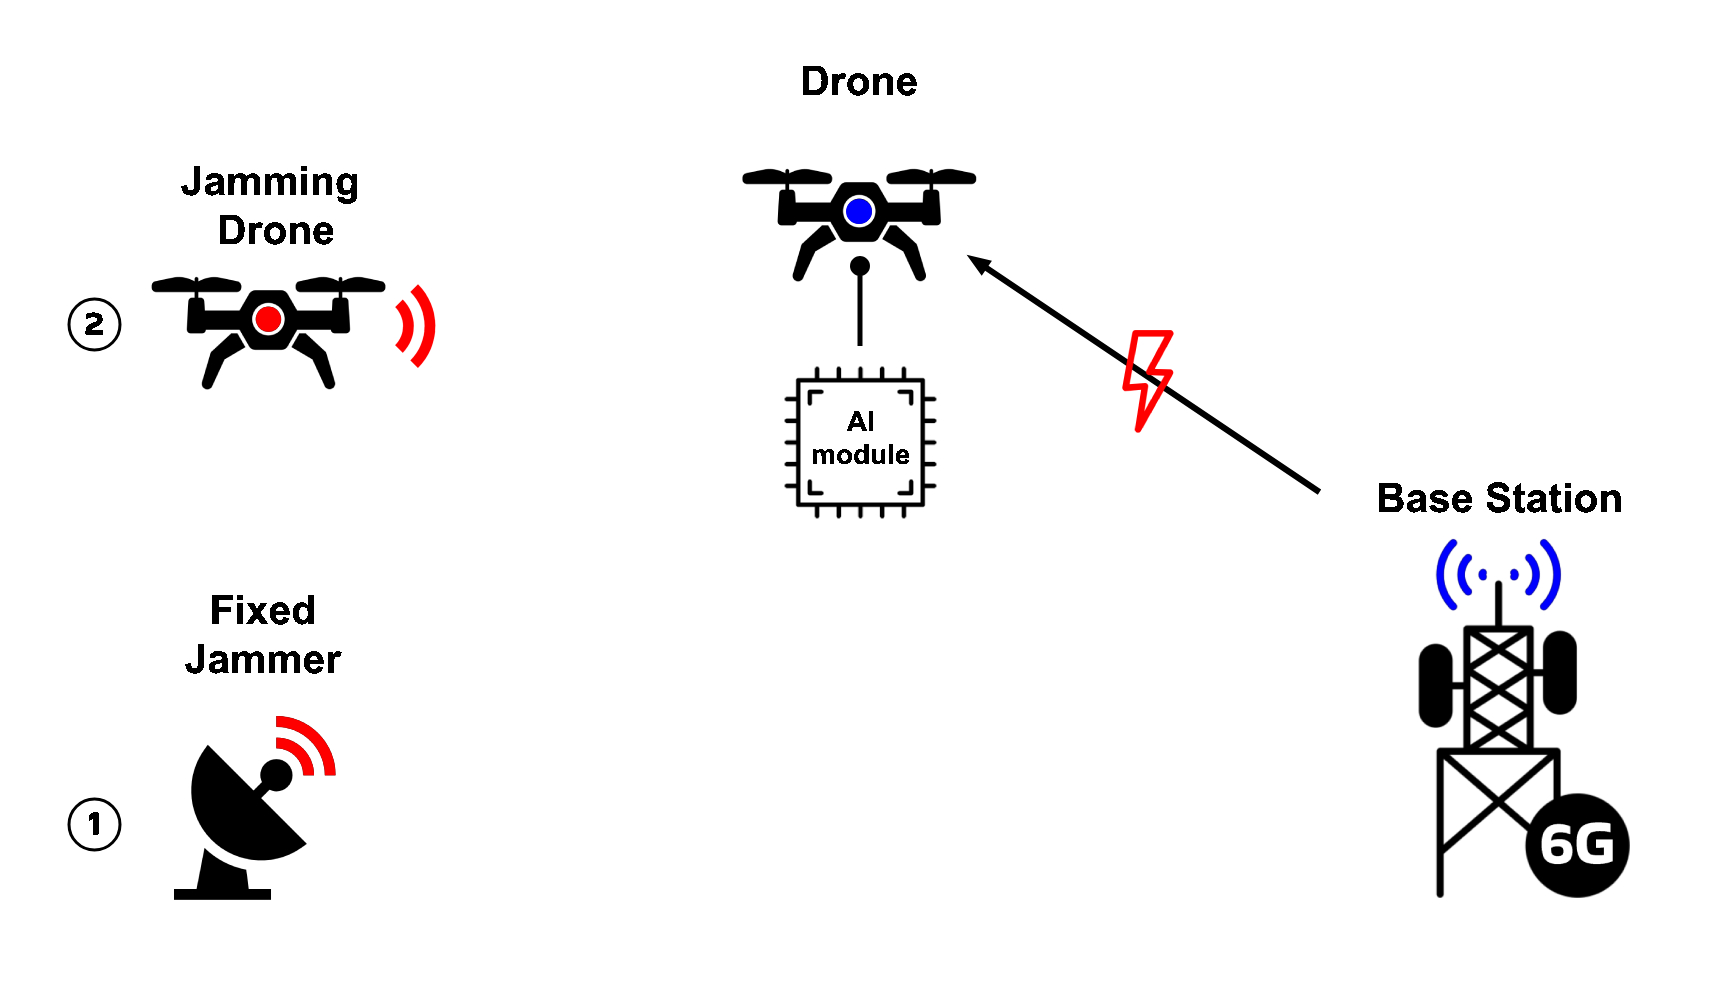
\includegraphics[width=10.5 cm]{img/CombinedJammingscenariosDiagram.jpg}
	\caption{Proposed jamming scenario. The Drone communicates with the 6G base station and receives information about how to behave. The fixed jammer \textbf{(1)} and the mobile jammer \textbf{(2)} target the communication between the drone and the base station. The drone has an internal classification module that is able to detect jamming attacks.}
	\label{fig:CombinedJammingscenariosDiagram}
	\end{figure}   
	\unskip


In our scenario, the drone will be subject to two types of jamming attacks, a constant jamming attack and a periodic jamming attack.
These types of attacks can be attributed to different types of jammers. The constant jamming attack could be caused by a ground jammer, as maintaining a constant jamming signal requires a large power source, while 
the periodic jamming attack could be caused by a drone jammer, as drones are usually battery powered and can only jam for a limited amount of time. 
Employing a periodic jamming attack could help the malicious drone conserve energy and reduce the chances of being detected.

Table \ref{tab:attacker_classification} shows the attacker classification in the proposed scenario \cite{MLMisbehavior5GBoualouache}: 

\begin{table}[H]
	\caption{Attacker classification details.\label{tab:attacker_classification}}
	\newcolumntype{C}{>{\centering\arraybackslash}X}
	\begin{tabularx}{\textwidth}{CC}
	\toprule
	\textbf{Classification} & \textbf{Description} \\
	\midrule
	Active   & The attacker is actively trying to disrupt network operation by transmitting a jamming signal\\
	External & The attack takes place at level 1 of the OSI model, meaning that the attacker is not part of the network\\
	Local    & The attack is local, as it is targeted at a specific drone or drone cluster and not at the entire network\\
	Malicious & Jamming attacks are considered malicious as their main goal is to disrupt correct network operation\\
	\bottomrule
\end{tabularx}
\end{table}

\subsection{Dataset Choice}

As 6G network traffic is not yet available, we chose an open-source dataset \cite{JammingDetectionIoT-Hussain} that analyses the RSS values 
received by a Raspberry Pi 3 that is subject to periodic and constant jamming attacks. 

The dataset was created using a software-defined radio (SDR) connected to a laptop that was programmed to transmit a jamming signal using the 
open source software \textit{GNU Radio}. A second SDR radio was chosen to receive the jamming signal and the RSS values and was connected 
to a Raspberry Pi 3. The jamming radio operates at a frequency of 2.412 GHz with a Bandwidth of 40MHz, while the Raspberry Pi 3 was programmed to sample the RSS values with a 
frequency of 32K samples per second. 

The dataset contains 3 different \textit{.txt} files that store the RSS values sampled by the Raspberry Pi 3. The first file contains the RSS values sampled during a constant jamming attack, the second file contains the RSS values sampled during a periodic jamming attack and the third file contains the RSS values sampled during normal network operation.
The samples are stored in a single column, with each row representing a single sample. The samples us the \textit{dBm (decibel-milliwatts)} unit of measurement a logarithmic scale that measures the power of a signal in relation to 1 milliwatt. 
Conversion can be done using the formula \cite{WirelessCommSobot} shown in equation \ref{eq:dbm_to_mw}:

\begin{linenomath}
	\begin{equation}
		P_{dBm} = 10 \cdot \log_{10} \left( \frac{P_{mW}}{1mW} \right)
		\label{eq:dbm_to_mw}
	\end{equation}
\end{linenomath}

Figures \ref{fig:ConstantJammingSignal} and \ref{fig:PeriodicJammingSignal} show respectively plots of the RSS values sampled during a constant jamming attack and a periodic jamming attack. 

\begin{figure}[H]
	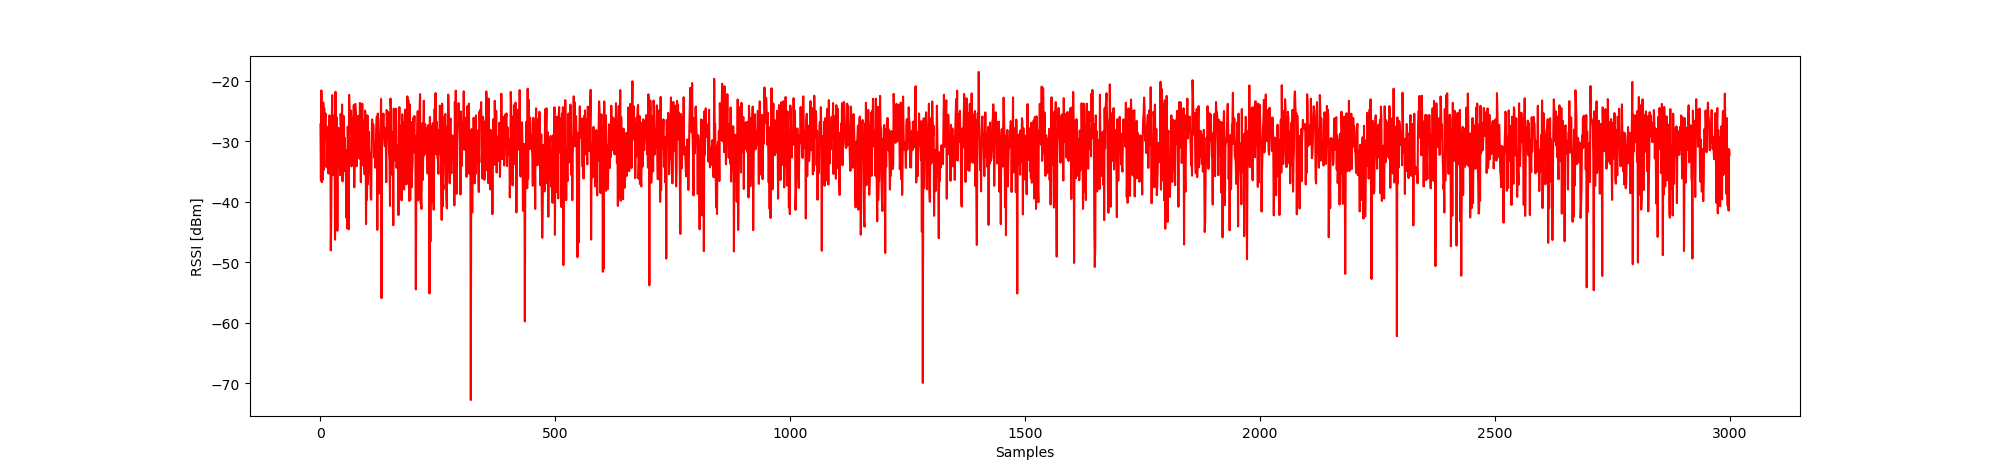
\includegraphics[width=10.5 cm]{img/ConstantJammingSignal.png}
	\caption{Constant jamming attack RSS values}
	\label{fig:ConstantJammingSignal}
\end{figure}   
\unskip
\begin{figure}[H]
	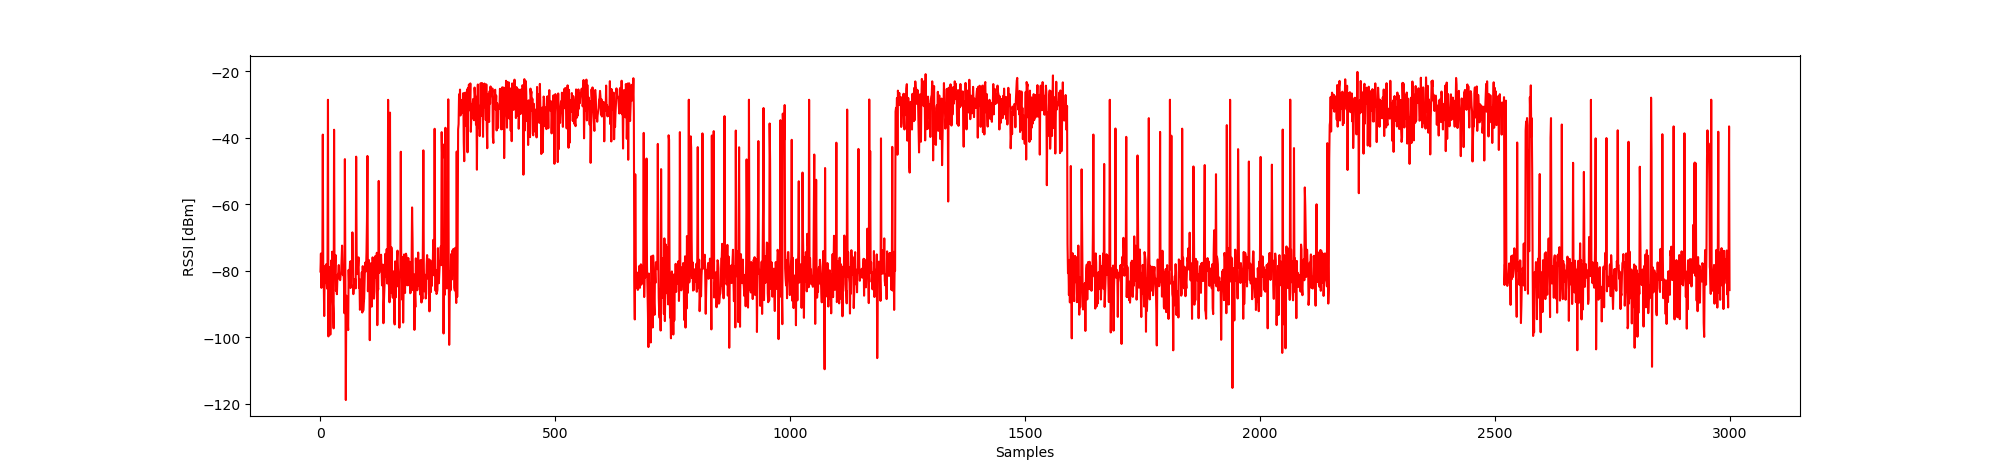
\includegraphics[width=10.5 cm]{img/PeriodicJammingSignal.png}
	\caption{Periodic jamming attack RSS values}
	\label{fig:PeriodicJammingSignal}
\end{figure}   
\unskip

\subsection {Algorithm Choice}

When choosing the algorithm for the classification module, we first had to define the requirements that the algorithm had to meet. The algorithm has to be able to classify anomalous samples with a high degree of accuracy, while at the same time 
being lightweight enough to be run on a resource constrained device like a drone. The training phase should also be fast, as this would allow the drone to redetermine the normal transmission RSS values in a constantly changing environment. If the model didn't periodically redefine normal RSS values, 
it would be prone to false positives caused by the mobile nature of drones. 
The model should be also required a limited amount of storage to be run effectively, as drones are usually lacking in internal storage. 

The algorithm that best fit these requirements was the \textit{Isolation Forest} algorithm \cite{IsolationForestLiu}. The Isolation Forest algorithm is a state-of-the-art unsupervised machine learning algorithm for anomaly detection, introduced by Liu et al. in 2008. 
Unlike traditional anomaly detection algorithms, which require the definition of a normal class, Isolation Forest is able to detect anomalies without explicitly defining the characteristics of the normal class.
This is achieved by leveraging the properties of anomalies themselves, i.e being few and separated from the majority of the data points. 
The algorithm works by building a forest of isolation trees. Each tree is built by randomly selecting one of the features and then splitting the data points based on a value randomly selected between the minimum and maximum value of the feature. This partitions the data into the 
left and right branches of the tree. The process is repeated recursively until all the data points are isolated. The height of a node, meaning the number of splits that were required to isolate is used to determine the anomaly score of the data point. The higher the number of splits, the more likely the data point is to be an anomaly.
Isolation Forest is an \textit{ensamble} algorithm, meaning that the final anomaly score is calculated by averaging the anomaly scores of all the trees in the forest. More trees mean more accuracy but also more computational power required.

\begin{figure}[H]
	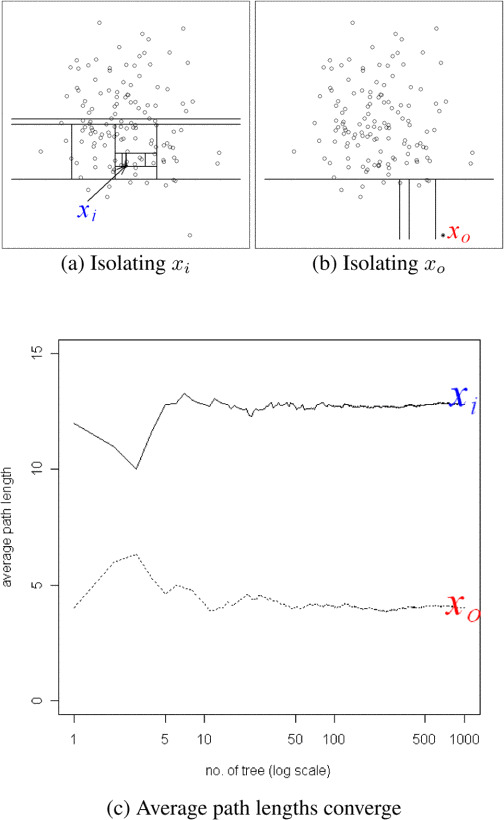
\includegraphics[width=6 cm]{img/IsolationForest.jpg}
	\caption{Isolation forest in action. The anomaly \textbf{x0} is isolated in less splits compared to the normal datapoint \textbf{x1}\cite{IsolationForestLiu}.}
	\label{fig:IsolationForest}
\end{figure}   
\unskip

The chosen implementation for isolation forest is the one provided by the \textit{Scikit-learn} library \cite{IsolationForestScikitLearn} for Python 3. 
The algorithm was tested on a Desktop PC with an Intel i7-6700 CPU and 16GB of RAM as well as on a Raspberry Pi 3 with a Quad Core 1.2GHz CPU and 1GB of RAM \cite{RaspberryPi3ModelB}.
The graphs shown are the ones obtained on the Desktop PC for convenience,  but the ability of the algorithm to run effectively on a resource constrained device like the Raspberry Pi 3, that has hardware comparable to the one found in high-end commercial drones, was verified. 

\subsection{Evaluation Metrics}\label{EvaluationMetrics}

The performance of the model was evaluated using the state-of-the-art evaluation metrics for machine learning classification algorithms. The metrics are all based on the number of true positives, false positives, true negatives and false negatives. A true positive is a data point that is correctly classified as an anomaly, while a false positive is a data point that is incorrectly classified as an anomaly. A true negative on the other hand is a data point that is correctly classified as a normal data point, while a false negative is a data point that is incorrectly classified as a normal data point.
The evaluation metrics that we chose to use are the following: 

\begin{itemize}
	\item \textbf{Accuracy:} The accuracy is the ratio of correctly classified data points to the total number of data points \ref{eq:accuracy}.
	\begin{equation}
		\label{eq:accuracy}
	  Accuracy = \frac{TP + TN}{TP + TN + FP + FN}
	\end{equation}
	\item \textbf{Precision:} The precision is the ratio of correctly classified anomalies to the total number of data points classified as anomalies \ref{eq:precision}.
	\begin{equation}
		\label{eq:precision}
	  Precision = \frac{TP}{TP + FP}
	\end{equation}
	\item \textbf{Recall:} The recall is the ratio of correctly classified anomalies to the total number of anomalies \ref{eq:recall}.
	\begin{equation}
		\label{eq:recall}
	  Recall = \frac{TP}{TP + FN}
	\end{equation}
	\item \textbf{F1 Score:} The F1 score is the harmonic mean of the precision and recall \ref{eq:f1}.
	\begin{equation}
		\label{eq:f1}
	  F1 = 2 \times \frac{Precision \times Recall}{Precision + Recall}
	\end{equation}
\end{itemize}

The combination of these metrics gives us an insight into the model's performance. 

%%%%%%%%%%%%%%%%%%%%%%%%%%%%%%%%%%%%%%%%
\section{Results}

\subsection{Parameters Tuning}

The first phase in our testing methodology was the tuning of the hyperparameters of the model. The tuning was performed by making the parameters vary between a minimum and a maximum value, evaluating the impact on the performance metrics (see section \ref{EvaluationMetrics}) and then choosing the best performing parameters.
From the parameters available in the \textit{Scikit-learn} implementation of the Isolation Forest, the parameters we decided to tune were the following: 

\begin{itemize}
	\item \textbf{n\_estimators:} The number of base estimators in the ensamble, i.e the number of isolation trees used to compute the anomaly score of each datapoint. 
	\item \textbf{max\_samples:} The max number of samples to draw from the dataset to train each tree.
	\item \textbf{contamination:} The amount of outliers present in the dataset used to train the model. 
\end{itemize}

During the tuning phase, the untested hyperparameters were set to their default values of the \textit{Scikit-learn} implementation of the Isolation Forest (\ref{tab:isolation_forest_parameters}).

\begin{table}[H]
	\caption{Scikit-Learn Isolation Forest hyperparameters default values.\label{tab:isolation_forest_parameters}}
	\newcolumntype{C}{>{\centering\arraybackslash}X}
	\begin{tabularx}{\textwidth}{CC}
	\toprule
	\textbf{Parameter} & \textbf{Default Value} \\
	\midrule
	n\_estimators & 100 \\
	max\_samples & 'auto' \\
	contamination & 0.1 \\
	\bottomrule
	\end{tabularx}
\end{table}

During he tuning process, as well as the subsequent model testing phase, the model was evaluated using as input normal traffic samples concatenated with jamming attack samples (see code snippet \ref{alg:dataset_concatenation}). 
This was done to simulate a real-world scenario where the model has to be able to classify correctly anomalous samples but also reduce the number of false positives during normal operation. 

\begin{algorithm}
	\caption{Test input definition}\label{alg:dataset_concatenation}
	\begin{algorithmic}[1]
	\State normalTraffic $\gets$ ReadAndParseFile(NORMAL\_TRAFFIC\_FILE, normal\_traffic\_size)
	\State jamming $\gets$ ReadAndParseFile(JAMMING\_FILE, jamming\_size)

	\State testInput $\gets$ Concatenate(normalTraffic, jamming)
	\end{algorithmic}
\end{algorithm}

The values whe chose for \textit{normal\_traffic\_size} and \textit{jamming\_size} are shown in table \ref{tab:dataset_sizes}. 

\begin{table}[H]
	\caption{Dataset sizes used for the tuning and testing phases.}\label{tab:dataset_sizes}
	\newcolumntype{C}{>{\centering\arraybackslash}X}
	\begin{tabularx}{\textwidth}{CC}
	\toprule
	\textbf{Dataset} & \textbf{Size} \\
	\midrule
	jamming samples n. & 2000 \\
	nominal samples n. & 20000 \\
	\bottomrule
\end{tabularx}
\end{table}

The dataset is purposefully unbalanced, as jamming attacks are usually rare events compared to normal network operation. 

In figure \ref{fig:InputSignal} we can see a representation of the input signal in the case of a constant jamming attack. The proposed results, unless otherwise specified, are based on the input signal shown in the figure which employs constant jamming. Periodic jamming always showed comparable trends as constant jamming in all the tests performed.


\begin{figure}[H]
	\begin{adjustwidth}{-\extralength}{0cm}
	\centering
	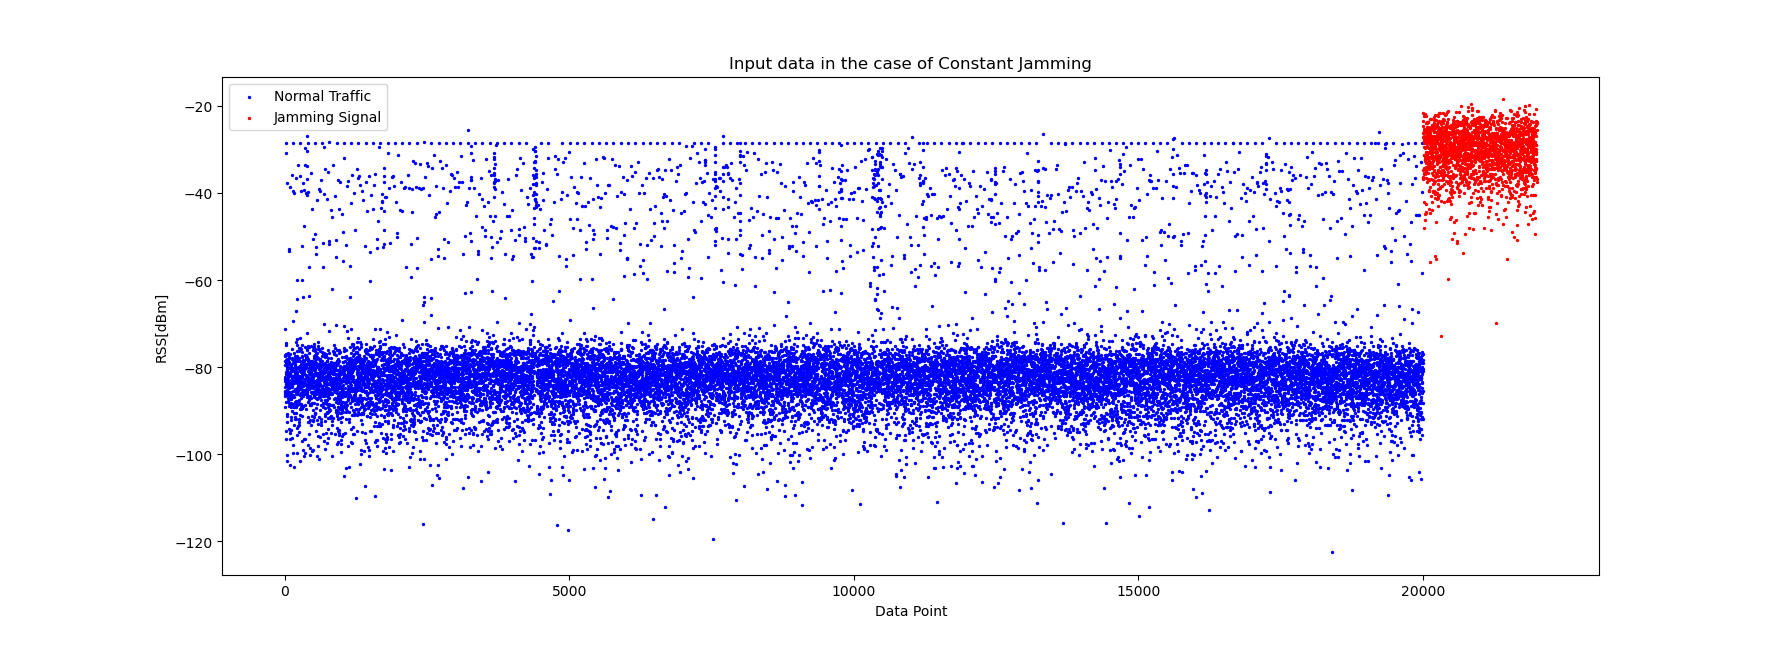
\includegraphics[width=19.5cm]{img/InputSignal.png}
	\caption{Input signal in the case of Constant Jamming. The jamming signal is concatenated with the normal traffic signal.}\label{fig:InputSignal}
\end{adjustwidth}
\end{figure}  

\subsubsection{n\_estimators tuning}

The first parameter that we decided to tune was the \textit{n\_estimators} parameter. The tuning values are shown in table \ref{tab:n_estimators_tuning}.

\begin{table}[H]
	\caption{n\_estimators tuning values.}\label{tab:n_estimators_tuning}
	\newcolumntype{C}{>{\centering\arraybackslash}X}
	\begin{tabularx}{\textwidth}{CC}
	\toprule
	\textbf{n\_estimators} & \textbf{Values} \\
	\midrule
	Minimum & 1 \\
	Maximum & 50 \\
	Step & 1 \\
	\bottomrule
\end{tabularx}
\end{table}

The effect on the evaluation metrics of the model is shown in figure \ref{fig:n_estimators_tuning}.

\begin{figure}[H]
	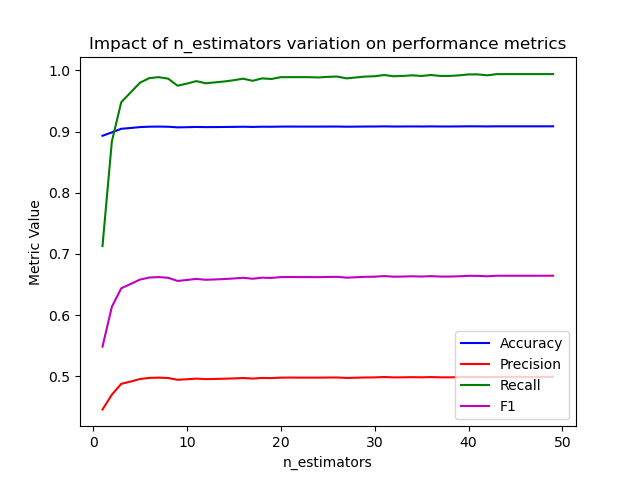
\includegraphics[width=10.5cm]{img/nEstimatorsTuning.png}
	\caption{n\_estimators tuning results.}\label{fig:n_estimators_tuning}
\end{figure}
\unskip

As we can see from the graph, a growing number of estimators initially correlates with a better model performance, but after a certain point the performance stabilizes. 
In graphs \ref{fig:n_estimators_training_time} and \ref{fig:n_estimators_classification_time} is shown that the time required both for training and classification increases linearly with the number of estimators.
This means that choosing an appropriate number of estimators is crucial, as it can greatly affect the model performance. 

\begin{figure}[H]
    \centering
    \begin{subfigure}{0.45\textwidth}
        \centering
        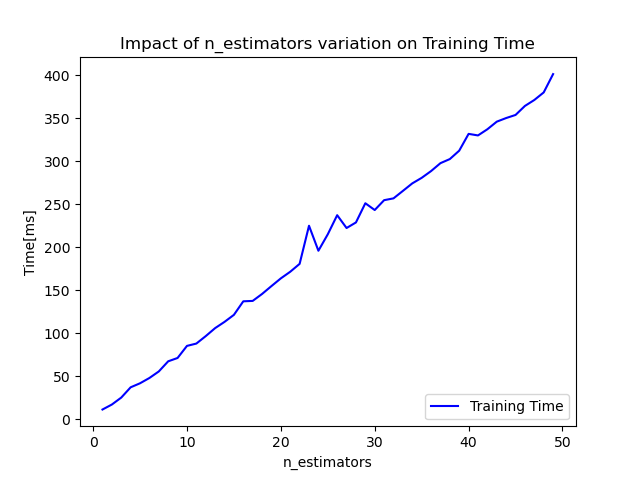
\includegraphics[width=\textwidth]{img/nEstimatorsTrainingTime.png}
        \caption{n\_estimators training time.}
        \label{fig:n_estimators_training_time}
    \end{subfigure}
    \hfill
    \begin{subfigure}{0.45\textwidth}
        \centering
        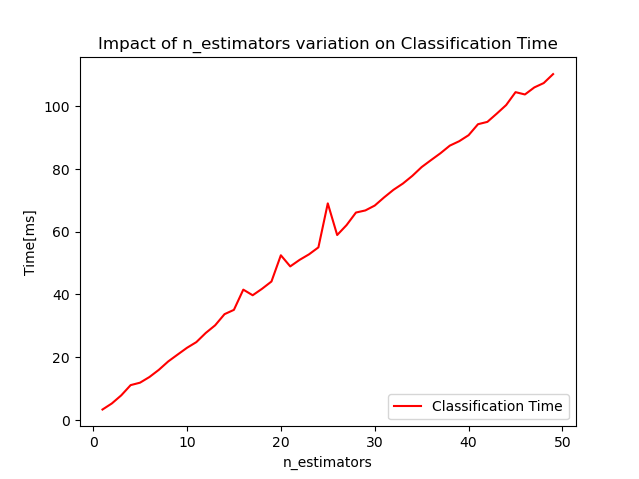
\includegraphics[width=\textwidth]{img/nEstimatorsClassificationTime.png}
        \caption{n\_estimators classification time.}
        \label{fig:n_estimators_classification_time}
    \end{subfigure}
    \caption{Comparison of n\_estimators training and classification times.}
    \label{fig:estimators_time_comparison}
\end{figure}


We decided to choose \textbf{n\_estimators = 15}, as it provided a good balance between model performance and computational resources required.
The model metrics keep slowly improving up until 45 estimators, but the minimal performance increase was not worth such a large increase in training and classification time, especially considering the resource-constrained nature of the scenario. 

\subsubsection{max\_samples tuning}

The second parameter that we decided to tune was the \textit{max\_samples} parameter. As shown in table \ref{tab:max_samples_tuning}, the tuning values were chosen to be between 1 and 20000, i.e the same number of normal traffic samples in the test input. 

\begin{table}[H]
	\caption{max\_samples tuning values.}\label{tab:max_samples_tuning}
	\newcolumntype{C}{>{\centering\arraybackslash}X}
	\begin{tabularx}{\textwidth}{CC}
	\toprule
	\textbf{max\_samples} & \textbf{Values} \\
	\midrule
	Minimum & 1 \\
	Maximum & 100 \\
	Step & 1 \\
	\bottomrule
\end{tabularx}
\end{table}

From figure \ref{fig:max_samples_tuning} we can see that the model performance is not greatly affected by the \textit{max\_samples} parameter. This is most likely due to the great difference in RSS values between the normal traffic samples and the jamming attack samples, meaning the model can develop the capability to correctly classify the input even with a small training set.

\begin{figure}[H]
	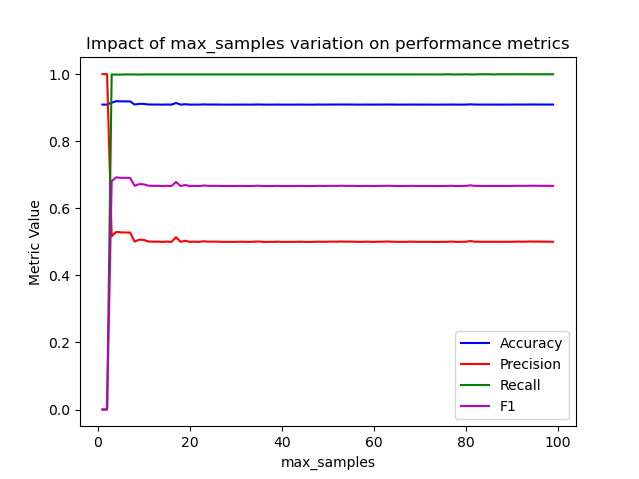
\includegraphics[width=10.5cm]{img/maxSamplesTuning.png}
	\caption{max\_samples tuning results.}\label{fig:max_samples_tuning}
\end{figure}
\unskip

Still, as the model has to build bigger trees, the \textit{max\_samples} parameters as considerable influence on the training and classification time, as shown in figure \ref{fig:max_samples_time_comparison}.
Given minimal performance differences but the impact on the time metrics, chose the value of \textbf{max\_samples = 10}. 

\begin{figure}[H]
	\centering
	\begin{subfigure}{0.45\textwidth}
		\centering
		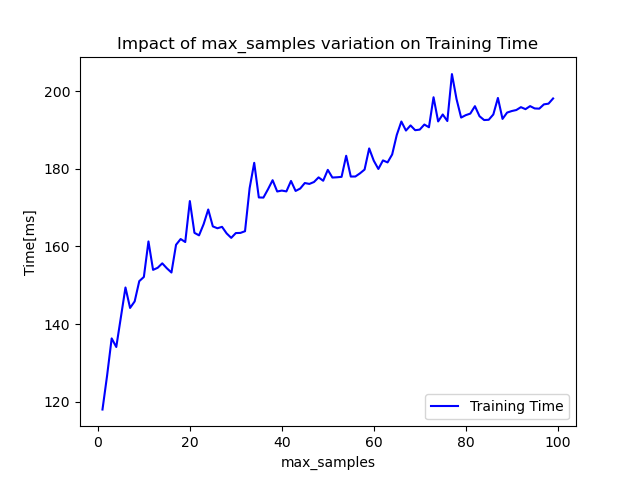
\includegraphics[width=\textwidth]{img/maxSamplesTrainingTime.png}
		\caption{max\_samples training time.}
		\label{fig:max_samples_training_time}
	\end{subfigure}
	\hfill
	\begin{subfigure}{0.45\textwidth}
		\centering
		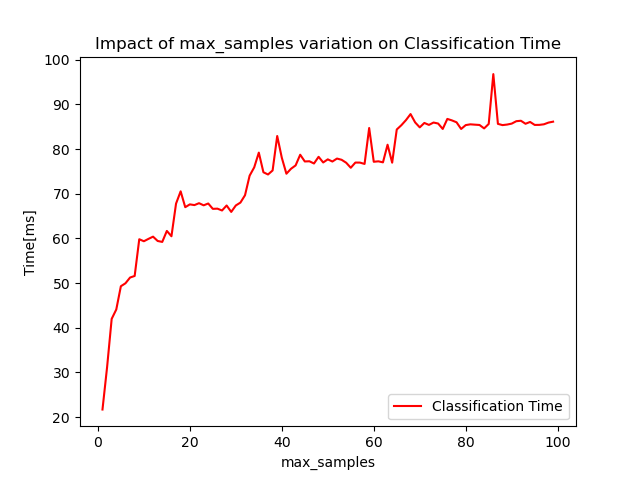
\includegraphics[width=\textwidth]{img/maxSamplesClassificationTime.png}
		\caption{max\_samples classification time.}
		\label{fig:max_samples_classification_time}
	\end{subfigure}
	\caption{Comparison of max\_samples training and classification times.}
	\label{fig:max_samples_time_comparison}
\end{figure}



%%%%%%%%%%%%%%%%%%%%%%%%%%%%%%%%%%%%%%%%%%
\section{Discussion}

Authors should discuss the results and how they can be interpreted from the perspective of previous studies and of the working hypotheses. The findings and their implications should be discussed in the broadest context possible. Future research directions may also be highlighted.

%%%%%%%%%%%%%%%%%%%%%%%%%%%%%%%%%%%%%%%%%%
\section{Conclusions}

This section is not mandatory, but can be added to the manuscript if the discussion is unusually long or complex.

%%%%%%%%%%%%%%%%%%%%%%%%%%%%%%%%%%%%%%%%%%
\section{Patents}

This section is not mandatory, but may be added if there are patents resulting from the work reported in this manuscript.

%%%%%%%%%%%%%%%%%%%%%%%%%%%%%%%%%%%%%%%%%%
\vspace{6pt} 
%%%%%%%%%%%%%%%%%%%%%%%%%%%%%%%%%%%%%%%%%%
\authorcontributions{For research articles with several authors, a short paragraph specifying their individual contributions must be provided. The following statements should be used ``Conceptualization, X.X. and Y.Y.; methodology, X.X.; software, X.X.; validation, X.X., Y.Y. and Z.Z.; formal analysis, X.X.; investigation, X.X.; resources, X.X.; data curation, X.X.; writing---original draft preparation, X.X.; writing---review and editing, X.X.; visualization, X.X.; supervision, X.X.; project administration, X.X.; funding acquisition, Y.Y. All authors have read and agreed to the published version of the manuscript.'', please turn to the  \href{http://img.mdpi.org/data/contributor-role-instruction.pdf}{CRediT taxonomy} for the term explanation. Authorship must be limited to those who have contributed substantially to the work~reported.}

\funding{Please add: ``This research received no external funding'' or ``This research was funded by NAME OF FUNDER grant number XXX.'' and  and ``The APC was funded by XXX''. Check carefully that the details given are accurate and use the standard spelling of funding agency names at \url{https://search.crossref.org/funding}, any errors may affect your future funding.}

\institutionalreview{In this section, you should add the Institutional Review Board Statement and approval number, if relevant to your study. You might choose to exclude this statement if the study did not require ethical approval. Please note that the Editorial Office might ask you for further information. Please add “The study was conducted in accordance with the Declaration of Helsinki, and approved by the Institutional Review Board (or Ethics Committee) of NAME OF INSTITUTE (protocol code XXX and date of approval).” for studies involving humans. OR “The animal study protocol was approved by the Institutional Review Board (or Ethics Committee) of NAME OF INSTITUTE (protocol code XXX and date of approval).” for studies involving animals. OR “Ethical review and approval were waived for this study due to REASON (please provide a detailed justification).” OR “Not applicable” for studies not involving humans or animals.}

\informedconsent{Any research article describing a study involving humans should contain this statement. Please add ``Informed consent was obtained from all subjects involved in the study.'' OR ``Patient consent was waived due to REASON (please provide a detailed justification).'' OR ``Not applicable'' for studies not involving humans. You might also choose to exclude this statement if the study did not involve humans.

Written informed consent for publication must be obtained from participating patients who can be identified (including by the patients themselves). Please state ``Written informed consent has been obtained from the patient(s) to publish this paper'' if applicable.}

\dataavailability{We encourage all authors of articles published in MDPI journals to share their research data. In this section, please provide details regarding where data supporting reported results can be found, including links to publicly archived datasets analyzed or generated during the study. Where no new data were created, or where data is unavailable due to privacy or ethical restrictions, a statement is still required. Suggested Data Availability Statements are available in section ``MDPI Research Data Policies'' at \url{https://www.mdpi.com/ethics}.} 

% Only for journal Nursing Reports
%\publicinvolvement{Please describe how the public (patients, consumers, carers) were involved in the research. Consider reporting against the GRIPP2 (Guidance for Reporting Involvement of Patients and the Public) checklist. If the public were not involved in any aspect of the research add: ``No public involvement in any aspect of this research''.}

% Only for journal Nursing Reports
%\guidelinesstandards{Please add a statement indicating which reporting guideline was used when drafting the report. For example, ``This manuscript was drafted against the XXX (the full name of reporting guidelines and citation) for XXX (type of research) research''. A complete list of reporting guidelines can be accessed via the equator network: \url{https://www.equator-network.org/}.}

% Only for journal Nursing Reports
%\useofartificialintelligence{Please describe in detail any and all uses of artificial intelligence (AI) or AI-assisted tools used in the preparation of the manuscript. This may include, but is not limited to, language translation, language editing and grammar, or generating text. Alternatively, please state that “AI or AI-assisted tools were not used in drafting any aspect of this manuscript”.}

\acknowledgments{In this section you can acknowledge any support given which is not covered by the author contribution or funding sections. This may include administrative and technical support, or donations in kind (e.g., materials used for experiments).}

\conflictsofinterest{Declare conflicts of interest or state ``The authors declare no conflicts of interest.'' Authors must identify and declare any personal circumstances or interest that may be perceived as inappropriately influencing the representation or interpretation of reported research results. Any role of the funders in the design of the study; in the collection, analyses or interpretation of data; in the writing of the manuscript; or in the decision to publish the results must be declared in this section. If there is no role, please state ``The funders had no role in the design of the study; in the collection, analyses, or interpretation of data; in the writing of the manuscript; or in the decision to publish the results''.} 

\abbreviations{Abbreviations}{
The following abbreviations are used in this manuscript:\\

\noindent 
\begin{tabular}{@{}ll}
SDN & Software Defined Networks\\
UAVs & Unmanned Aerial Vehicles \\
3GPP & 3rd Generation Partnership Project \\
V2X & Vehicle to Everything \\
FPV & First Person View \\
DOS & Denial Of Service \\
SNR & Signal to Noise Ratio \\
RSSI & Received Signal Strength Indicator \\
PDR & Packet Delivery Ratio \\
CIA & Confidentiality, Integrity, Availability \\
IoT & Internet of Things \\
AI & Artificial Intelligence \\
DSSS & Direct Sequence Spread Spectrum \\
FHSS & Frequency Hopping Spread Spectrum \\
OSI & Open Systems Interconnection \\
dBm & Decibel-milliwatts \\


\end{tabular}
}

%%%%%%%%%%%%%%%%%%%%%%%%%%%%%%%%%%%%%%%%%%
%% Optional
\appendixtitles{no} % Leave argument "no" if all appendix headings stay EMPTY (then no dot is printed after "Appendix A"). If the appendix sections contain a heading then change the argument to "yes".
\appendixstart
\appendix
\section[\appendixname~\thesection]{}
\subsection[\appendixname~\thesubsection]{}
The appendix is an optional section that can contain details and data supplemental to the main text---for example, explanations of experimental details that would disrupt the flow of the main text but nonetheless remain crucial to understanding and reproducing the research shown; figures of replicates for experiments of which representative data are shown in the main text can be added here if brief, or as Supplementary Data. Mathematical proofs of results not central to the paper can be added as an appendix.

\begin{table}[H] 
\caption{This is a table caption.\label{tab5}}
\newcolumntype{C}{>{\centering\arraybackslash}X}
\begin{tabularx}{\textwidth}{CCC}
\toprule
\textbf{Title 1}	& \textbf{Title 2}	& \textbf{Title 3}\\
\midrule
Entry 1		& Data			& Data\\
Entry 2		& Data			& Data\\
\bottomrule
\end{tabularx}
\end{table}

\section[\appendixname~\thesection]{}
All appendix sections must be cited in the main text. In the appendices, Figures, Tables, etc. should be labeled, starting with ``A''---e.g., Figure A1, Figure A2, etc.

%%%%%%%%%%%%%%%%%%%%%%%%%%%%%%%%%%%%%%%%%%
\begin{adjustwidth}{-\extralength}{0cm}
%\printendnotes[custom] % Un-comment to print a list of endnotes

\reftitle{References}

% Please provide either the correct journal abbreviation (e.g. according to the “List of Title Word Abbreviations” http://www.issn.org/services/online-services/access-to-the-ltwa/) or the full name of the journal.
% Citations and References in Supplementary files are permitted provided that they also appear in the reference list here. 

%=====================================
% References, variant A: external bibliography
%=====================================
%\bibliography{your_external_BibTeX_file}

%=====================================
% References, variant B: internal bibliography
%=====================================
\begin{thebibliography}{999}

\bibitem[Taylor(2024)]{5GStatisticsTaylor}
5G - statistics \& facts. Available online: \url{https://www.statista.com/topics/3447/5g/topicOverview} (accessed on 13 September 2024).

\bibitem[Letaief et al.(2019)]{6GRoadmapLetaief}
Letaief, K.B.; Chen, W.; Shi, Y.; Zhang, J.; AI, B. The Roadmap to 6G: AI Empowered Wireless Networks. {\em IEEE Communications Magazine} {\bf 2019}, {\em 57}, 84--90. \url{https://doi.org/10.1109/MCOM.2019.1900271}.

\bibitem[EuropeanCommission(2024)]{DronesEC}
Unmanned aircraft (drones). Available online: \url{https://transport.ec.europa.eu/transport-modes/air/aviation-safety/unmanned-aircraft-drones_en} (accessed on 13 September 2024).

\bibitem[Laricchia(2024)]{DronesStatisticsLaricchia}
Laricchia, F. Consumer and commercial drones - statistics and facts. Available online: \url{https://www.statista.com/topics/7939/drones/\#topicOverview} (accessed on 13 September 2024).

\bibitem[Sultan(2018)]{5GV2XSultan}
Sultan, A. Study on enhancement of 3GPP support for 5G V2X services. Tech. Rep. {\em 3GPP}, 2018.

\bibitem[Hassija et al.(2021)]{DroneCommHassija}
Hassija, V.; Kumar, R.; Gupta, H.; Singh, S.; Sharma, P. Fast, Reliable, and Secure Drone Communication: A Comprehensive Survey. {\em IEEE Communications Surveys and Tutorials} {\bf 2021}, {\em 23}, 2802--2832. \url{https://doi.org/10.1109/COMST.2021.3097916}.

\bibitem[Rao et al.(2024)]{DroneCombatUkraine}
Rao, A.; Zafra, M.; Hunder, M.; Kiyada, S. How drone combat in Ukraine is changing warfare. Available online: \url{https://www.reuters.com/graphics/UKRAINE-CRISIS/DRONES/dwpkeyjwkpm/} (accessed on 13 September 2024).

\bibitem[Cawthra(2020)]{DataIntegrityCawthra}
Cawthra, J. Data Integrity: Detecting and Responding to Ransomware and Other Destructive Events. {\em NIST Special Publication} {\bf 2020}, {\em 1800-26A}.

\bibitem[Lyamin et al.(2018)]{VANETsAI-Lyamin}
Lyamin, N.; Samuylov, A.; Gaidamaka, Y.; Vinel, A.; Koucheryavy, Y. AI-Based Malicious Network Traffic Detection in VANETs. {\em IEEE Network} {\bf 2018}, {\em 32}, 15--21. \url{https://doi.org/10.1109/MNET.2018.1800074}.

\bibitem[Boualouache and Engel(2023)]{MLMisbehavior5GBoualouache}
Boualouache, A.; Engel, T. A Survey on Machine Learning-Based Misbehavior Detection Systems for 5G and Beyond Vehicular Networks. {\em IEEE Communications Surveys and Tutorials} {\bf 2023}, {\em 25}, 1128--1172. \url{https://doi.org/10.1109/COMST.2023.3236448}.

\bibitem[Feng and Haykin(2019)]{AntiJammingV2V-Feng}
Feng, S.; Haykin, S. Cognitive Risk Control for Anti-Jamming V2V Communications in Autonomous Vehicle Networks. {\em IEEE Transactions on Vehicular Technology} {\bf 2019}, {\em 68}, 9920--9934. \url{https://doi.org/10.1109/TVT.2019.2935999}.

\bibitem[Owano(2024)]{RQ170DroneOwano}
Owano, N. RQ-170 drone's ambush facts spilled by Iranian engineer. Available online: \url{https://phys.org/news/2011-12-rq-drone-ambush-facts-iranian.html} (accessed on 14 September 2024).

\bibitem[Gross and TOI Staff(2024)]{IranianUAVGross}
Gross, J.A.; TOI Staff. Iranian UAV that entered Israeli airspace seems to be American stealth knock-off. Available online: \url{https://www.timesofisrael.com/iranian-uav-that-enteredisraeli-airspace-seems-to-be-american-stealth-knock-off} (accessed on 16 May 2024).

\bibitem[Chorti et al.(2022)]{6GSecurity-Chorti}
Chorti, A.; Hollanti, C.; Koorapaty, H.; Poor, H.V. Context-Aware Security for 6G Wireless: The Role of Physical Layer Security. {\em IEEE Communications Standards Magazine} {\bf 2022}, {\em 6}, 102--108. https://doi.org/10.1109/MCOMSTD.0001.2000082.

\bibitem[Sciancalepore et al.(2023)]{JammingDetection-Sciancalepore}
Sciancalepore, S.; Kusters, F.; Abdelhadi, N.K.; Oligeri, G. Jamming Detection in Low-BER Mobile Indoor Scenarios via Deep Learning. {\em arXiv} {\bf 2023}, eprint: 2306.10912. Available online: \url{https://arxiv.org/abs/2306.10912}.

\bibitem[Boualouache and Engel(2023)]{MLMisbehavior5GBoualouache}
Boualouache, A.; Engel, T. A Survey on Machine Learning-Based Misbehavior Detection Systems for 5G and Beyond Vehicular Networks. {\em IEEE Communications Surveys and Tutorials} {\bf 2023}, {\em 25}, 1128--1172. https://doi.org/10.1109/COMST.2023.3236448.

\bibitem[Hussain et al.(2023)]{JammingDetectionIoT-Hussain}
Hussain, A.; Zhang, M.; Bhatia, S.; Cheng, L. Jamming Detection in IoT Wireless Networks: An Edge-AI Based Approach. In Proceedings of the 12th International Conference on the Internet of Things, IoT ’22; Association for Computing Machinery: Delft, Netherlands, 2023; pp. 57--64. ISBN: 9781450396653. https://doi.org/10.1145/3567445.3567456.

\bibitem[Sobot(2012)]{WirelessCommSobot}
Sobot, R. \textit{Wireless Communication Electronics: Introduction to RF Circuits and Design}; Springer: 2012; p. 252. ISBN 9783030486303.

\bibitem[Liu et al.(2008)]{IsolationForestLiu}
Liu, F.T.; Ting, K.M.; Zhou, Z.-H. Isolation Forest. In Proceedings of the 2008 Eighth IEEE International Conference on Data Mining, Pisa, Italy, 2008; pp. 413--422. https://doi.org/10.1109/ICDM.2008.17.

\bibitem[Scikit-learn(2024)]{IsolationForestScikitLearn}
Scikit-learn: Isolation Forest. Available online: \url{https://scikit-learn.org/stable/modules/generated/sklearn.ensemble.IsolationForest.html} (accessed on 14 September 2024).

\bibitem[RaspberryPi(2024)]{RaspberryPi3ModelB}
Raspberry Pi 3 Model B. Available online: \url{https://www.raspberrypi.com/products/raspberry-pi-3-model-b/} (accessed on 14 September 2024).


\end{thebibliography}

% If authors have biography, please use the format below
%\section*{Short Biography of Authors}
%\bio
%{\raisebox{-0.35cm}{\includegraphics[width=3.5cm,height=5.3cm,clip,keepaspectratio]{Definitions/author1.pdf}}}
%{\textbf{Firstname Lastname} Biography of first author}
%
%\bio
%{\raisebox{-0.35cm}{\includegraphics[width=3.5cm,height=5.3cm,clip,keepaspectratio]{Definitions/author2.jpg}}}
%{\textbf{Firstname Lastname} Biography of second author}

% For the MDPI journals use author-date citation, please follow the formatting guidelines on http://www.mdpi.com/authors/references
% To cite two works by the same author: \citeauthor{ref-journal-1a} (\citeyear{ref-journal-1a}, \citeyear{ref-journal-1b}). This produces: Whittaker (1967, 1975)
% To cite two works by the same author with specific pages: \citeauthor{ref-journal-3a} (\citeyear{ref-journal-3a}, p. 328; \citeyear{ref-journal-3b}, p.475). This produces: Wong (1999, p. 328; 2000, p. 475)


\PublishersNote{}
\end{adjustwidth}
\end{document}

